\documentclass{article}

\usepackage{graphicx}
\usepackage{tikz}
\usepackage{tikzsymbols}
\usetikzlibrary{calc,patterns,shapes.geometric}
\pagestyle{empty}
\usepackage[margin=0pt]{geometry}
\geometry{papersize={14in,12in}}

\def\centerarc[#1](#2)(#3:#4:#5){\draw[#1] ($(#2)+({#5*cos(#3)},{#5*sin(#3)})$) arc (#3:#4:#5);}

\begin{document}
	\begin{figure}
		\centering
		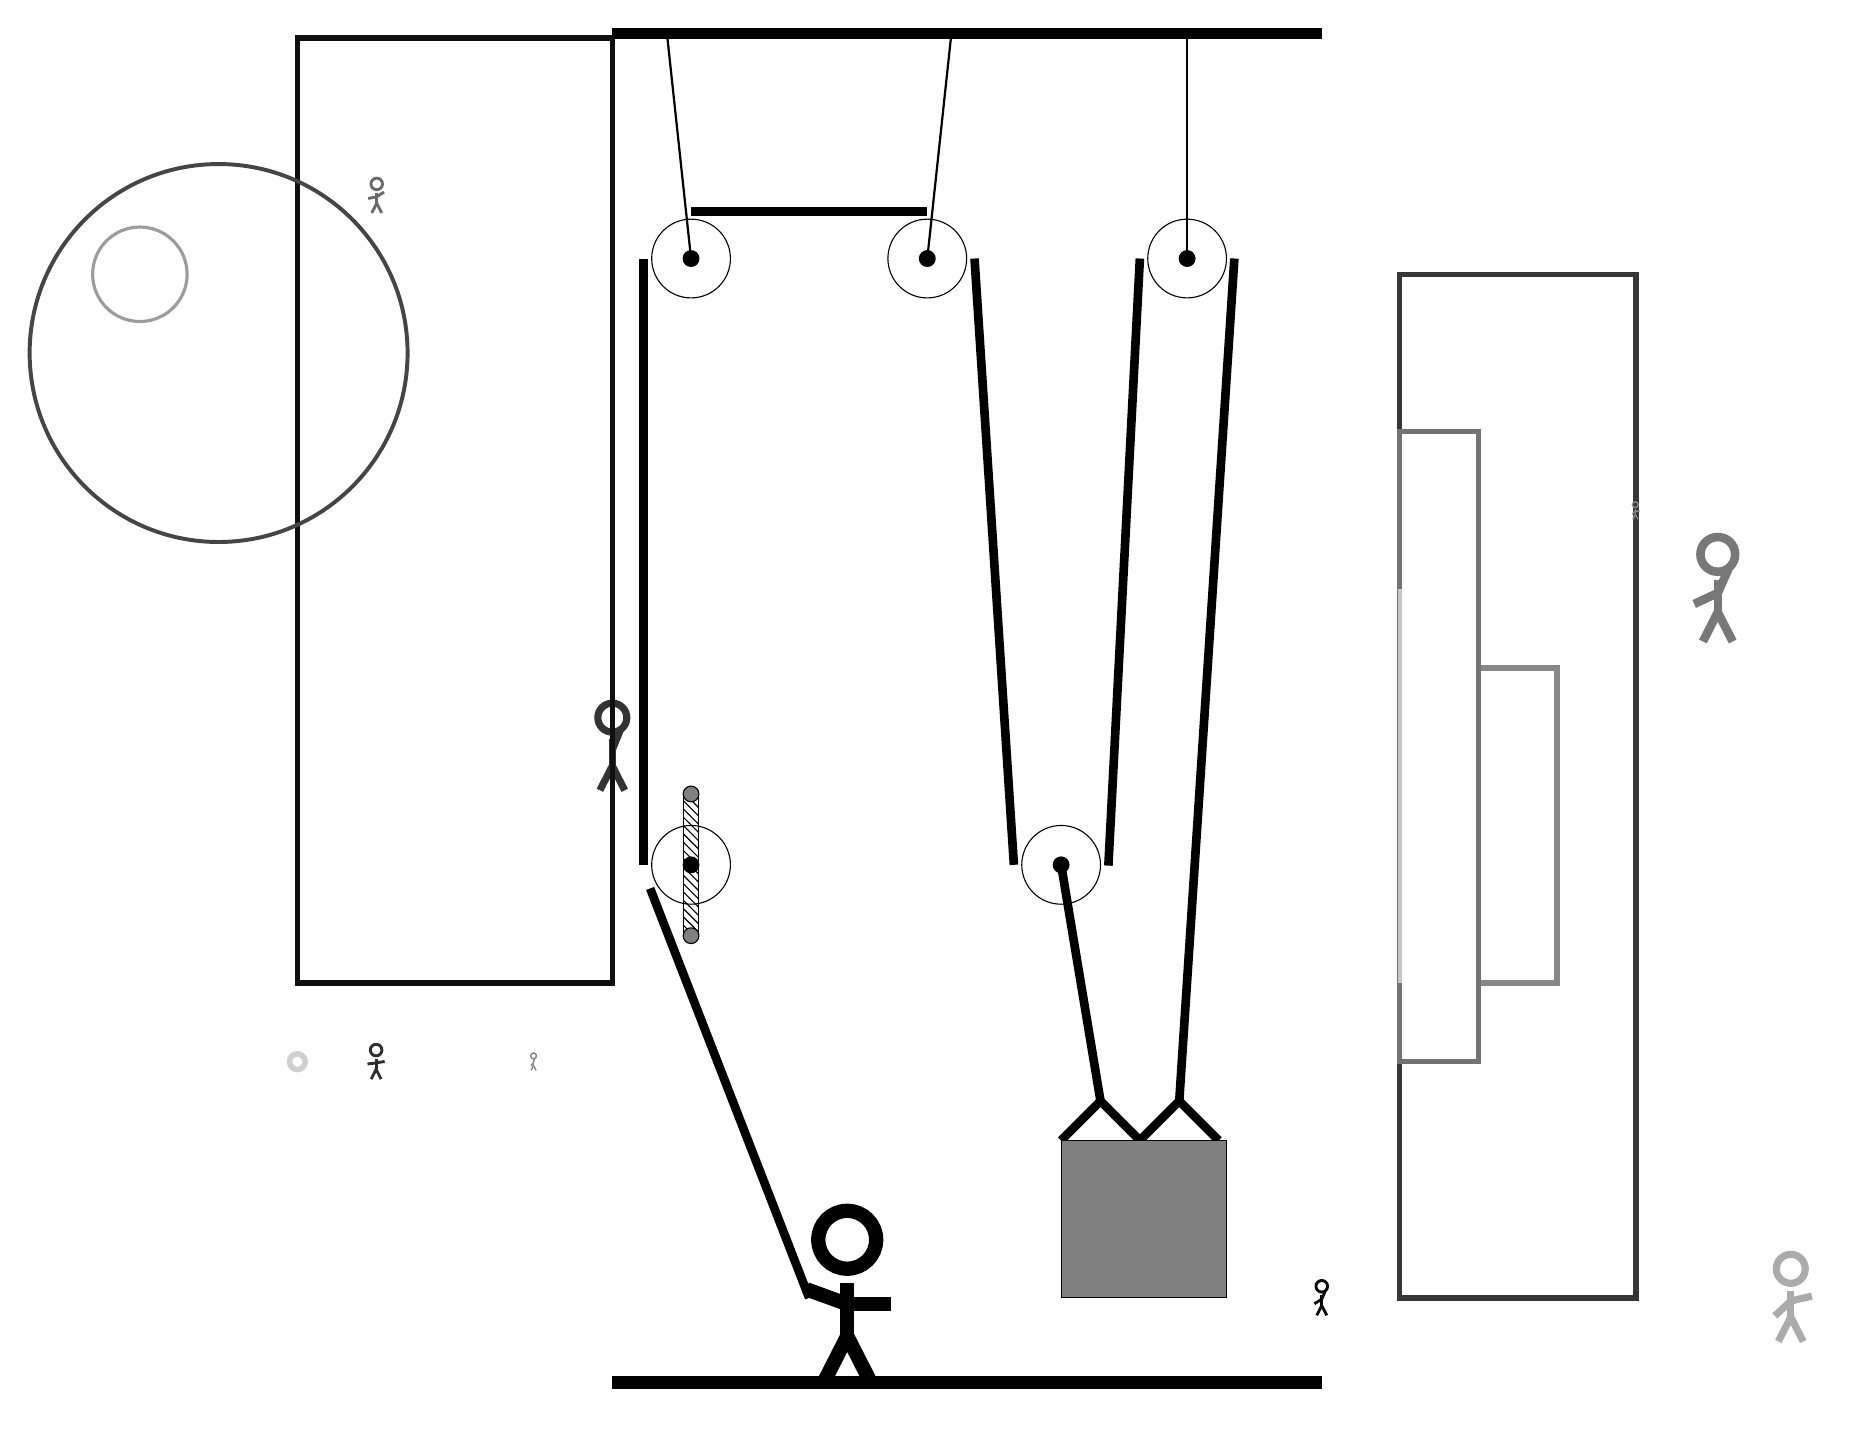
\begin{tikzpicture}
			%%%%% START %%%%%
			
			\draw[fill=black] (-3, 14) rectangle (6, 14.125);
			
			\draw (1, 11.2) circle (0.5);
			\draw[fill=black] (1, 11.2) circle (0.1);
			\draw[thick] (1, 11.2) -- (1.3, 14);
			
			\draw (4.3, 11.2) circle (0.5);
			\draw[fill=black] (4.3, 11.2) circle (0.1);
			\draw[thick] (4.3, 11.2) -- (4.3, 14);
			
			\draw (2.7, 3.5) circle (0.5);
			\draw[fill=black] (2.7, 3.5) circle (0.1);
			
			\draw[line width=1.1mm]  (2.7, 0) -- (3.2, 0.5) -- (3.7, 0) -- (4.2, 0.5) -- (4.7, 0);
			\draw[fill=black!50] (2.7, 0) rectangle (4.8, -2);
			
			\draw (-2, 11.2) circle (0.5);
			\draw[fill=black] (-2, 11.2) circle (0.1);
			\draw[thick] (-2, 11.2) -- (-2.3, 14);
			
			\draw (-2, 3.5) circle (0.5);
			\draw[fill=black] (-2, 3.5) circle (0.1);
			\draw[pattern=north west lines, pattern color=black] (-2.1, 4.4) rectangle (-1.9, 2.6);
			\draw[fill=black!50] (-2, 4.4) circle (0.1);
			\draw[fill=black!50] (-2, 2.6) circle (0.1);
			
			\node[line width=0.2mm, color=black!97] at (6, -2) {\Strichmaxerl[2][32][67]};
			
			\draw[line width=0.7mm, color=black!47] (8, 6) rectangle (9, 2);
			\draw[line width=0.7mm, color=black!79] (7, -2) rectangle (10, 11);
			\node[line width=0.7mm, color=black!59] at (-6, 12) {\Strichmaxerl[2][11][33]};
			\draw[line width=0.6mm, color=black!55] (7, 9) rectangle (8, 1);
			\node[line width=0.7mm, color=black!47] at (10, 8) {\Strichmaxerl[1][44][1]};
			\draw [line width=0.4mm, color=black!39](-9, 11) circle (0.6);
			
			\node[line width=0.4mm, color=black!80] at (-3, 5) {\Strichmaxerl[5][90][68]};
			\node[line width=0.3mm, color=black!33] at (12, -2) {\Strichmaxerl[5][43][13]};
			\draw [line width=0.7mm, color=black!19](-7, 1) circle (0.1);
			
			\draw [line width=0.4mm, color=black!92](-7, 14) circle (0.0);
			\draw[line width=0.7mm, color=black!94] (-3, 14) rectangle (-7, 2);
			\node[line width=0.7mm, color=black!82] at (-6, 1) {\Strichmaxerl[2][7][10]};
			\draw [line width=0.5mm, color=black!73](-8, 10) circle (2.4);
			\node[line width=0.4mm, color=black!53] at (11, 7) {\Strichmaxerl[6][25][66]};
			\node[line width=0.7mm, color=black!48] at (-4, 1) {\Strichmaxerl[1][57][78]};
			
			\draw[line width=0.5mm, color=black!22] (7, 7) rectangle (7, 2);
			
			\draw[line width=1.1mm](-0.5, -2) -- (-2.5196, 3.2);
			\centerarc[line width=1.1mm](-2, 3.5)(180:210:0.6);
			\draw[line width=1.1mm](-2.6, 3.5) -- (-2.6, 11.2);
			\centerarc[line width=1.1mm](-2, 11.2)(90:180:0.6);
			
			\draw[line width=1.1mm](-2, 11.8) -- (1, 11.8);
			\centerarc[line width=1.1mm](1, 11.2)(0:90:0.6);
			\draw[line width=1.1mm](1.6, 11.2) -- (2.1, 3.5);
			\centerarc[line width=1.1mm](2.7, 3.5)(180:370:0.6);
			\draw[line width=1.1mm] (3.3, 3.49) -- (3.7, 11.2);
			\centerarc[line width=1.1mm](4.3, 11.2)(0:180:0.6);
			\draw[line width=1.1mm](4.2, 0.5) -- (4.9, 11.2);
			\draw[line width=1.1mm] (3.2, 0.5) -- (2.7, 3.5);
			
			\node at (0, -2) {\Strichmaxerl[10][-20][0]};
			
			\draw[fill=black] (-3, -3) rectangle (6, -3.15);
			
			%%%%% END %%%%%
		\end{tikzpicture}
	\end{figure}	
\end{document}